\title{PostgreSQL y yo}
\newcommand{\putcollection}{
  \put(0,10){
    \parbox{\textwidth}{
      \fontsize{30}{30}\selectfont
      Álvaro Herrera \\
      PostgreSQL developer -- 2ndQuadrant Inc.\\
      UbuCon LA, agosto 2019
    }
  }
}
\newcommand{\insertcopyright}{}
\renewcommand{\insertcopyright}{(C) 2ndQuadrant Limited 2008-2019}
\date{}

\begin{document}

  \begin{frame}[plain]
    \titlepage
  \end{frame}

\begin{frame}
\frametitle{Sobre 2ndQuadrant}

\begin{itemize}
\item Empresa de servicios y soporte a PostgreSQL
\item Auspiciador de la comunidad PostgreSQL
\item Desarrolladores de características principales de PostgreSQL
\item https://www.2ndQuadrant.com/
\end{itemize}

\vfill
\hfill  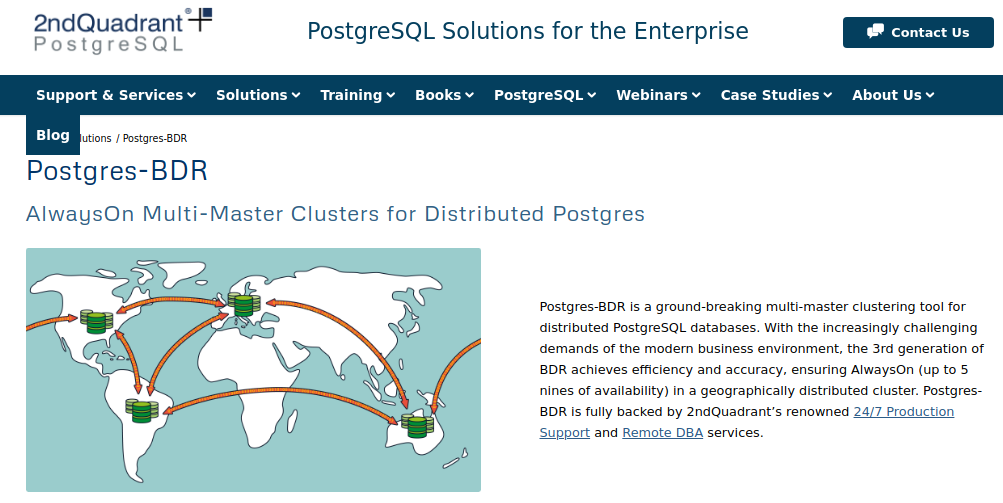
\includegraphics[width=0.6\textwidth]{2ndq-website.png}

\end{frame}

\begin{frame}
\frametitle{Sobre Álvaro Herrera}

\begin{itemize}
\item Desarrollador de PostgreSQL desde 2002
\item Committer de PostgreSQL desde 2005
\end{itemize}

\end{frame}

\begin{frame}
 \frametitle{Qué es PostgreSQL}

\begin{itemize}
\item Sistema de almacenamiento y manipulación de datos
\item Interoperable con otros DBMS: lenguaje SQL estándar
\item Confiable, consistente, robusto (ACID)
\item Potente, flexible, extensible
\item Excelente rendimiento, escalable a hardware muy grande
\end{itemize}
\end{frame}

\begin{frame}
 \frametitle{Características principales}

\begin{itemize}
\item Gran soporte de lenguaje SQL
\begin{itemize}
\item   Transacciones, savepoints
\item   INNER JOIN, OUTER JOIN
\item   UNION, INTERSECT, EXCEPT
\item   subconsultas
\item   agrupamiento, agregación
\item   INFORMATION\_SCHEMA
\item   WITH RECURSIVE
\item   Window functions (LAG, LEAD, ...)
\item   disparadores (triggers)
\item   SQL/XML, SQL/JSON
\end{itemize}
\end{itemize}
\end{frame}

\begin{frame}
  \frametitle{Características principales (cont.)}

  \begin{itemize}
    \item Extensiones
      \begin{itemize}
	\item Tipos de datos, métodos de índice, métodos de tabla
	\item \textit{background workers}
      \end{itemize}
    \item   resistencia a fallas frente a cortes abruptos de energía (WAL)
    \item   Replicación binaria, replicación lógica
    \item   ``hot standby''
    \item   Respaldos en caliente, respaldos continuos
    \item \textit{Foreign Data Wrappers}
  \end{itemize}

\end{frame}

\begin{frame}
  \frametitle{Herramientas de gestión}

  \begin{itemize}
    \item Consolas de administración
      \begin{itemize}
	\item https://OmniDB.org
      \end{itemize}
    \item Orquestación
      \begin{itemize}
	\item Patroni, de Zalando: https://github.com/zalando/patroni
      \end{itemize}
    \item Monitoreo
      \begin{itemize}
	\item Icinga, Zabbix, Prometheus, etc
      \end{itemize}
    \item Alta disponibilidad, balanceo de carga
  \end{itemize}
\end{frame}

\begin{frame}
  \frametitle{Licencia}

    \begin{itemize}
      \item The PostgreSQL License
	\begin{itemize}
	  \item MIT, BSD
	\end{itemize}
      \item Úsela todo lo que quiera
      \item No copyleft
	\begin{itemize}
      \item Derivados comerciales permitidos
	\end{itemize}
    \end{itemize}
\end{frame}

\begin{frame}
  \frametitle{PostgreSQL Global Development Group}

  \center 
\includegraphics{devmeet-2017.jpg}

\end{frame}

\begin{frame}
  \frametitle{Ranking DB-Engines.com}

 \fullsizegraphic{dbengines.png}
\end{frame}

\begin{frame}
  \begin{itemize}
    \item Mi propia historia
    \item Erase una vez ...
    \item ... un joven estudiante de ingeniería
  \end{itemize}
\end{frame}

\being{frame}
	\fullsizegraphic{Atentus.png}
\end{frame}

\begin{frame}
	\fullsizegraphic{firstpost.png}
\end{frame}

\begin{frame}
	\fullsizegraphic{corruptdb.png}
\end{frame}

\begin{frame}[containsverbatim]
 \frametitle{Un nombre en un commit}

\footnotesize
\begin{Verbatim}[xleftmargin=-0.7cm]
commit 087771ae4025238af8547819b01bb699c27fa593
Author:     Tom Lane <tgl@sss.pgh.pa.us>
AuthorDate: Tue Oct 23 02:20:15 2001 +0000
CommitDate: Tue Oct 23 02:20:15 2001 +0000
 
    Add error checking to PageRepairFragmentation to ensure that it can
    never overwrite adjacent pages with copied data, even if page header
    and/or item pointers are already corrupt.  Change inspired by trouble
    report from Alvaro Herrera.
\end{Verbatim}
\end{frame}

\begin{frame}
  \frametitle{Una aventura inesperada}
	\begin{itemize}
		\item Entretenciones de nerd:
			\begin{itemize}
				\item leer mensajes de commit
			\end{itemize}
		\item En ese tiempo era CVS
			\begin{itemize}
				\item Leer changelog era un parto
				\item (comparado con Git)
				\item mucho mejor que guardar $2^7$ copias versionando en el nombre de archivo
			\end{itemize}
	\end{itemize}
\end{frame}

\begin{frame}[containsverbatim]
  \frametitle{Un desafío en un commit}

\footnotesize
\begin{Verbatim}[xleftmargin=-0.7cm]
commit 565639cde0787f32e20e0b51591a7ad0a07c2aff
Author:     Tom Lane <tgl@sss.pgh.pa.us>
AuthorDate: Fri Jan 12 01:22:21 2001 +0000
CommitDate: Fri Jan 12 01:22:21 2001 +0000

    Preserve constraints and column defaults during CLUSTER.
    Wish they were all this easy ...
\end{Verbatim}
\end{frame}

\begin{frame}[containsverbatim]
  \frametitle{Un desafío en un commit (2)}

\footnotesize
\begin{Verbatim}[xleftmargin=-0.7cm]
commit 565639cde0787f32e20e0b51591a7ad0a07c2aff
Author:     Tom Lane <tgl@sss.pgh.pa.us>
AuthorDate: Fri Jan 12 01:22:21 2001 +0000
CommitDate: Fri Jan 12 01:22:21 2001 +0000

    Preserve constraints and column defaults during CLUSTER.
\end{Verbatim}
	\Huge
	\alert{\texttt{Wish they were all this easy ...}}
\end{frame}

\begin{frame}
	\center
	
\includegraphics[height=0.7\textheight]{Challenge-Accepted.jpg}
\end{frame}

\begin{frame}
  \frametitle{¿Cómo llegué a este punto?}

	\begin{itemize}
		\item Inglés
		\item Curiosidad
		\item Persistencia, dedicación, determinación
	\end{itemize}
\end{frame}

\begin{frame}
\fullsizegraphic{tgl.png}
\end{frame}

\begin{frame}
\fullsizegraphic{bmomjian.png}
\end{frame}

\begin{frame}[containsverbatim]
  \frametitle{\texttt{CLUSTER}}

\footnotesize
\begin{Verbatim}[xleftmargin=-1cm]
commit 7dc40a2be053a11544c708f576f2bb2858f14aa9
Author:     Bruce Momjian <bruce@momjian.us>
AuthorDate: Sat Aug 10 20:43:46 2002 +0000
CommitDate: Sat Aug 10 20:43:46 2002 +0000

    Major improvement in CLUSTER which preserves table characteristics using
    relfilenode.
    
    I sent the CLUSTER patch a few days ago and I think it was missed.  I
    append it again, this time including the regression test files.  For the
    committer, please note that you have to cvs add the files as they don't
    exist.  Maybe add to the parallel and serial schedules also, but I don't
    know such stuff.
    
    Alvaro Herrera (<alvherre[a]atentus.com>)

\end{Verbatim}
\end{frame}

\begin{frame}
  \frametitle{La tesis}

	\begin{itemize}
		\item Esto se convirtió en mi tema de tesis
		\item Lo más difícil:
			\begin{itemize}
				\item conseguir profesor auspiciante
			\end{itemize}
		\item Tres proyectos:
		\begin{itemize}
			\item Cluster
			\item re-indexamiento de btrees
			\item Savepoints
		\end{itemize}
	\end{itemize}
\end{frame}

\begin{frame}[containsverbatim]
  \frametitle{Savepoints}

\footnotesize
\begin{Verbatim}[xleftmargin=-1cm]
commit 573a71a5da70d6e2503c8f53e3b4f26b3b6d738d
Author:     Tom Lane <tgl@sss.pgh.pa.us>
AuthorDate: Thu Jul 1 00:52:04 2004 +0000
CommitDate: Thu Jul 1 00:52:04 2004 +0000

    Nested transactions.  There is still much left to do, especially on the
    performance front, but with feature freeze upon us I think it's time to
    drive a stake in the ground and say that this will be in 7.5.
    
    Alvaro Herrera, with some help from Tom Lane.
\end{Verbatim}
\end{frame}

\begin{frame}
  \frametitle{...}

	\begin{itemize}
		\item Afortunadamente, Savepoints quedó incompleto
		\item Bruce Momjian me ofreció \$\$ de Fujitsu para completarlo
	\end{itemize}

	\vfill
\small

PostgreSQL contributor.

Authored: autovacuum, background workers, BRIN indexes, commit timestamps, savepoints, shared row locking, some partitioning features.
  
Co-authored: DDL-event triggers, XMLTABLE, crosstabview, pluggable storage.

Solid sixteen years writing new PostgreSQL features, my code appears in all supported major releases and is used in millions of servers around the world.

Your database is corrupt? I can fix it.

\end{frame}

\begin{frame}
  \frametitle{Steve Jobs / Think Different}

Best marketing strategy ever! Steve Jobs Think different / Crazy ones speech

\center
  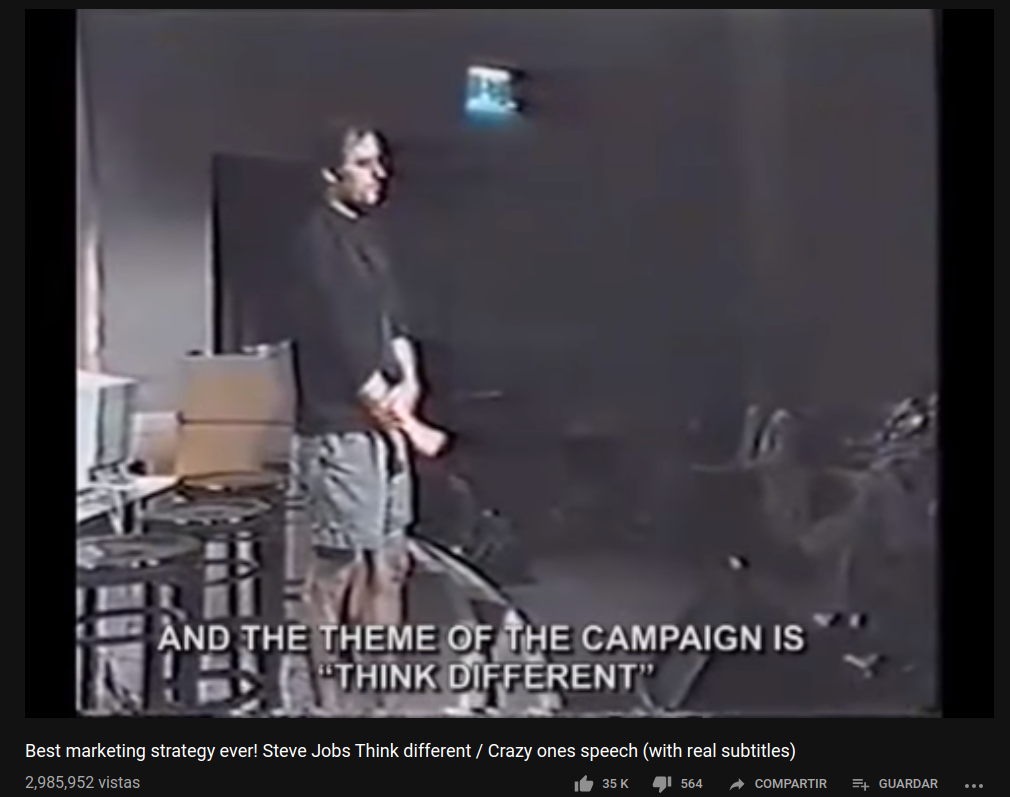
\includegraphics[height=0.7\textheight]{stevejobs.png}
  \url{https://www.youtube.com/watch?v=keCwRdbwNQY}

\end{frame}

\begin{frame}
  \frametitle{Grano de arena}

  \begin{itemize}
    \item Si cada uno aporta un granito de arena ...
      \pause
    \item Seis mil quinientos millones de granos de arena ...
      \pause
    ­\item Cada grano son 170 pL
    \item Caben en un balde
  \end{itemize}

\end{frame}

\begin{frame}
  \center 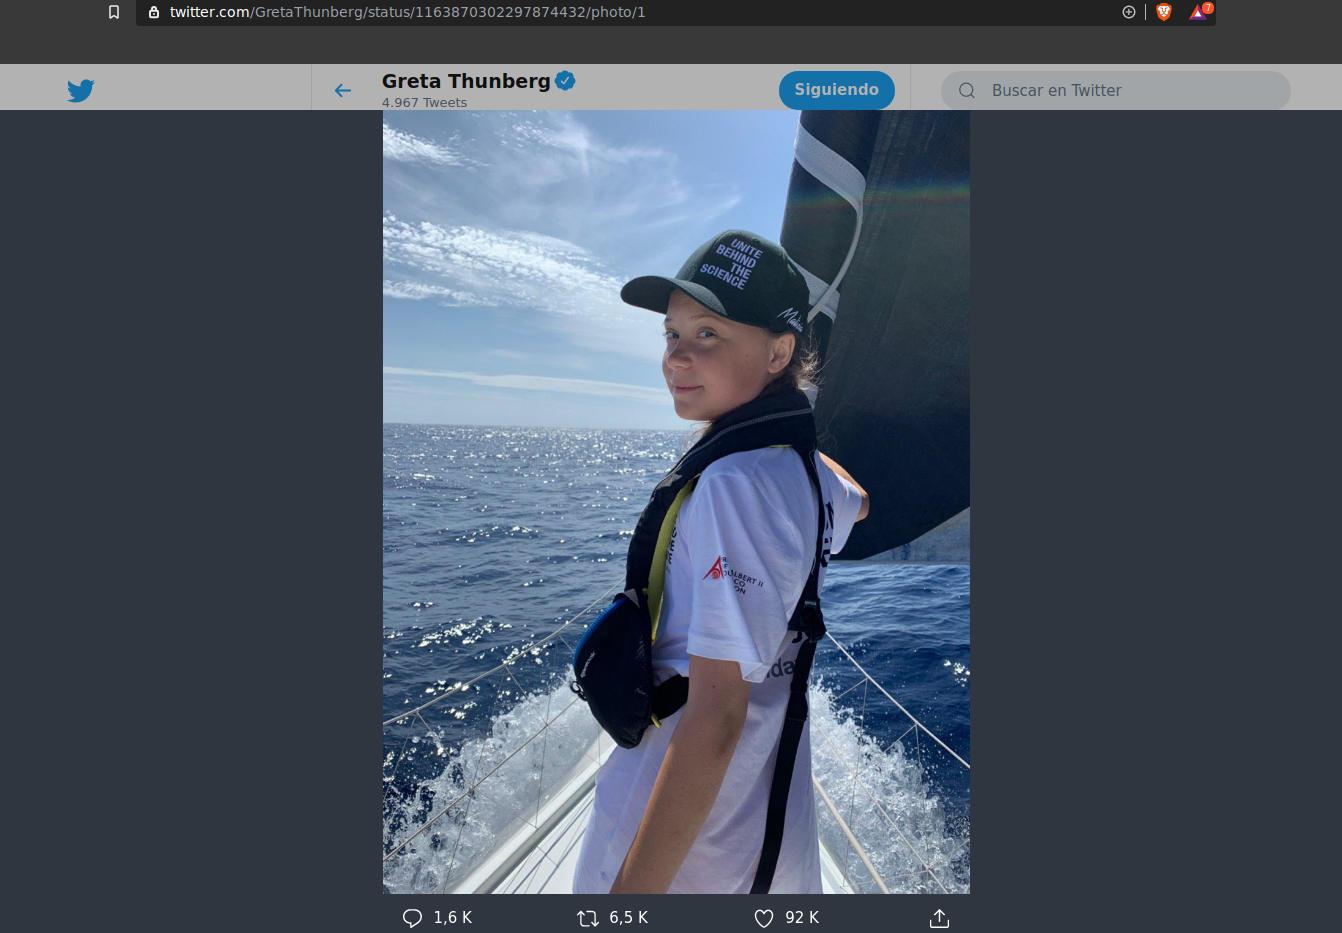
\includegraphics[height=\textheight]{greta.png}
\end{frame}

\begin{frame}
  \frametitle{¡Postgres Day Santiago!}

  \center 

  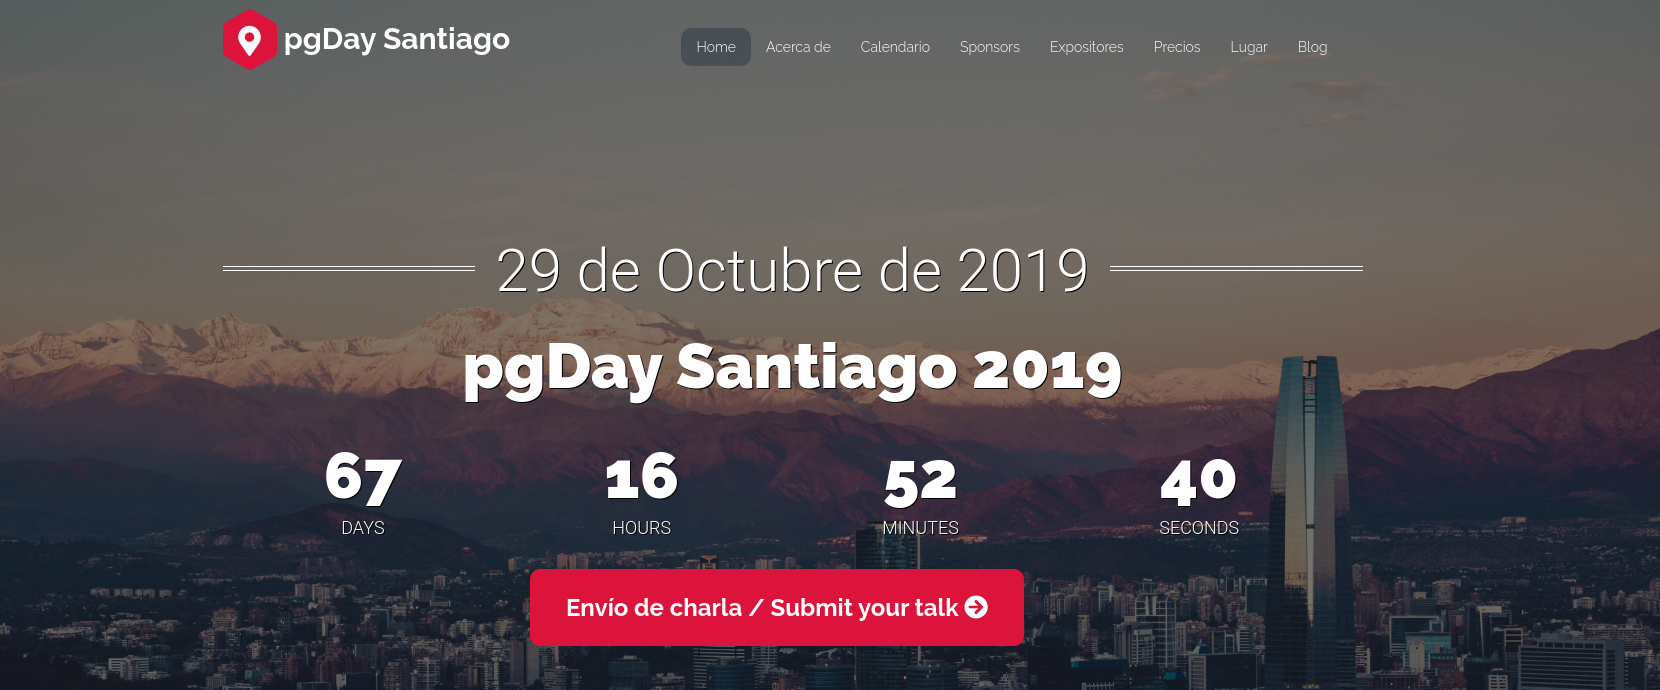
\includegraphics[height=0.7\textheight]{pgday.png}
\url{https://pgday.cl/2019/}
\end{frame}
